\section{Theoretische Vorbereitung}
    \subsection{Reziprokes Gitter}
        Das reziproke Gitter ist ein mathematisches Konstrukt, welches besonders geeignet ist um Beugung von Wellen
        an periodischem Gittern zu beschreiben, da es durch die Beugungen von Wellen an diesem bzw. durch die 
        Fouriertransformation beschrieben wird.
         Es wird häufig in Zusammenhang mit den Miller'schen Indizes verwendet
        um die Netzebenen $(hkl)$ zu beschreiben. Es bietet sich an diese im Reziproken zu definieren, da die Länge
        eines Vektors der die Position eines Gitterpunkts beschreibt gleich dem Reziproken des Abstands der
        Netzebenen entspricht.
        Aus den Basisvektoren des Punktgitter ($\vec{a_1},\vec{a_2},\vec{a_3}$) ergeben sich über folgende Beziehung
        die Basisvektoren ($\vec{b_1},\vec{b_2},\vec{b_3}$) des reziproken Gitters.
        \begin{align*}
            \vec{b_1} = 2\pi \frac{\vec{a_2}\times \vec{a_3}}{\vec{a_1}\cdot (\vec{a_2}\times \vec{a_3})}
            \\\vec{b_2} = 2\pi \frac{\vec{a_3}\times \vec{a_1}}{\vec{a_1}\cdot (\vec{a_2}\times \vec{a_3})}
            \\\vec{b_3} = 2\pi \frac{\vec{a_1}\times \vec{a_2}}{\vec{a_1}\cdot (\vec{a_2}\times \vec{a_3})}
        \end{align*}
        Über diese Definition der Basisvektoren lassen sich die Koordinaten eines Punktes im reziproken Gitter
        über die Miller'schen indizes $(hkl)$ beschreiben.
        
        \subsubsection*{Bragg Gleichung}
            Die Bragg Gleichung liefert einen Zusammenhang zwischen dem Netzebenenabstand $d_{hkl}$ und dem
            Beugungswinkel $\theta$. Damit dieser Zusammenhang gilt, muss jedoch der einfallende und gebeugte
            Strahl symmetrisch zur reflektierende Netzebene verlaufen. Damit die beiden Strahlen konstruktiv
            inteferieren können, muss der Wellenlängenunterschied $n\lambda$ betragen (destruktive $n\frac{\lambda}{2}$)
            Dann lässt sich der Zusammenhang beschreiben durch
            \begin{equation}
                n\lambda = 2d_{hkl} \sin(\theta)
            \end{equation}
            aus dieser lässt sich die äquivalente Laue Bedingung ableiten, welche aussagt,
            dass ein Röntgenstrahl genau dann gestreut wird, wenn der Beugungsvektor $\vec{k}$ gleich dem
            reziproken Gittervektor ist. 
    
    \subsection{Ordnungsparameter und Phasenübergänge}
        Bei einem Phasenübergang handelt es sich um eine Umwandlung einer Phase eines Stoffes in 
        eine andere Phase. Diese Übergänge treten meist in Abhängigkeit von einem oder mehrerer Zustandsvariablen
        wie Druck oder Temperatur auf.\\
        Will man nun den Zustand eines physikalischen Systems nicht nur vor und nach einem Übergang beschreiben,
        so dienen die Ordnungsparameter zur eben dieser. Geht man beispielsweise von einem Übergang von einer
        flüssigen in eine feste Phase, wie beispielweise bei Gefrierung von Wasser, so geht das System von einer
        hohen Symmetrie in eine Phase in der lediglich die Gittersymetrie verbleibt. Dieser Übergang lässt sich
        anhand des Ordnungsparameters als Übergang von absoluter Unordnung ($s=0$) zur absoluten Ordnung
        ($s=1$) beschreiben. Diese Beschreibung lässt sich auf beliebige Übergänge übertragen, bei denen
        gegebenenfalls kein eindeutiger Phasenwechsel auftritt, je nach dem verändert sich der Ordnungsparameter
        entweder plötzlich oder kontinuierlich. Nach der Ehrenfest Klassifikation gibt es Phasenübergänge erster Ordnung (plötzlicher Wechsel) und jene 
        höherer Ordnung (kontinuierliche Phasenübergänge).
        Anhand der Thermondynamik lässt sich über
        \begin{equation}
            F = E-TS
        \end{equation}
        (freie Energie F, Energie E, Temperatur T, Entropie S)\\
        zeigen, dass der Ordnungsparameter stehts versucht die freie Energie zu minimieren um schlussendlich
        einen Gleichgewichtszustand mit mininmaler freien Energie zu erreichen.

    \subsection{Überstrukturen}
        Eine Überstruktur beschreibt eine Elementarzelle die größer ist als die des Kristallgitters selbst.
        Nimmt man beispielsweise eine reine Oberfläche/Kristalline Struktur an, so
        gäbe es keine Überstrukturen, diese kommen erst dann zustande wenn beispielweise Adsorbatome an einer Oberfläche
        eine weiteres geordnetes Gitter bilden welches größer ist als das des reinen ursprünglichen Gitters.
        Überstrukturen werden nach Wood, über ein vielfaches der reziproken Gittervektoren angegeben, beispielweise
        \begin{align*}
            (2\times1) \text{  die Überstruktur ist in x-Richtung doppelt so groß wie die Elementar Zelle}\\
            (\sqrt{2}\times\sqrt{2})R45 \text{  um 45° rotierte quadratische Zelle[2]}
        \end{align*}
        Überstrukturen lassen sich beispielsweise direkt mit dem Rastertunnelmikroskop sichtbar machen.
        Andererseits lässt sich über Beugungsverfahren das reziproke Gitter der Oberfläche abbilden, bei der die
        Überstruktur zu anderen Periodizitäten im reziproken Gitter führt. Was sich in Form von zusätzlichen Beugungsmaxima 
        Beugungsmaxima bemerkbar macht.

        \subsection{Legierung}
            Eine Legierung ist ein Gemisch aus mindestens einem Metall (Basismetall) und einem anderen Element (Komponente). Im Allgemeinen 
            haben Legierungen einen kristallinen Aufbau. Die Legierung weist andere chemische Eigenschaften, wie Härte oder elektrische Leitfähigkeit,
            auf als das Basismetall. Künstliche Legierungen können dazu verwendet werden, um Werkstoffeigenschaften auf gewünschte Weise zu ändern.
        \subsubsection{$CuZn$ - Legierung}
            Die $CuZn$ Legierung (Messing) kristallisiert in einem bcc-Gitter. Beide Elemente kristallisieren in einem sc-Gitter,
            wobei die beiden Gitter so verschoben sind, dass in einer Zelle sich ein Eckatom des anderen Gitters befindet $\Rightarrow$ bcc-Gitter 
            
        \subsubsection{$CuAu$ - Legierung}
            Wird Kupfer und Gold zu gleichen Teilen gemischt, so bildet sich im ungeordneten Fall eine fcc-Struktur. Die Gitterplätze sind gleichermaßen
            mit Kupfer- und Goldatomen besetzt. Bei der geordneten Struktur sind in der $[001]$-Ebene die Gitterplätze abwechselnd von Kupfer- und Goldatomen besetzt.
            Durch diese abwechselnde Besetzung wird das fcc-Gitter verzerrt, so dass $\frac{\vec{a_3}}{\vec{a_1}} = 0.93$ beobachtet wird.

        \subsubsection{$Cu_3Au$ - Legierung}
            Wird nun Kupfer und Gold 3:1 gemischt, entsteht im ungeordneten Fall wieder ein fcc-Gitter, aber diesmal mit anderen Wahrscheinlichkeiten
            (75\% Kupfer-, 25\% Goldatome). Die geordnete Struktur ist nun deutlich komplizierter. Auf den ersten Blick sieht es wie ein fcc-Gitter aus, 
            jedoch zeichnet sich die $Cu_3Au$ Kristallstruktur dadurch aus, dass sowohl Gold als auch Kupfer in sc-Gittern kristallisieren. Somit liegen 
            vier sc-Gitter ineinander. Die Goldatome formen ein sc-Gitter, welches mit den bisherigen fcc-Gitter Eckatomen übereinstimmt.
            Die übrigbleibenden zentrierten Flächenplätze können nun durch  drei sc-Gitter von Kupferatomen beschrieben werden.
    \subsection{Die röntgenographische Methode}

        \subsubsection{Röntgenstrahlung}    
            Röntgenstrahlung gehört zum elektromagnetischen Spektrum und entspricht einer Energie von etwa
            100eV oder einer Wellenlänge $~10 nm$. In diesem Versuch benötigt man eine Wellenlänge von $\lambda \thicksim 0.1 nm$, da 
            die Wellenlaenge ungefaehr mit den Groessen der Streuobjekte uebereinstimmen muss. Es gibt unterschiedliche Möglichkeiten Röntgenstrahlung zu erzeugen. 
            Durch Elektronen kann Röntgenstrahlung erzeugt werden, bei starkem Beschleunigen (meist Abbremsen oder Umlenken) von Elektronen entsteht die sogenannte Bremsstrahlung, welche im Energiebereich
            von Röntgenstrahlung liegt. Somit lässt sich Röntgenstrahlung in einer Röntgenröhre ohne großen Aufwand erzeugen.
            Eine Röntgenröhre besteht aus einer evakuierten Röhre, einer Glühkathode und einer Anode. Bei der Glühkathode werden
            freie Elektronen erzeugt und durch einen Spannungsunterschied zur Anode hinbeschleunigt. Beim Auftreffen auf die Anode
            der Elektronen entsteht Röntgenstrahlung. Die erzeugte Röntgenstrahlung besteht aus zwei Komponenten, dem kontinuierlichen Spektrum
            und einem diskreten Linienspektrum. Das kontinuierliche Spektrum wird erzeugt, durch die unterschiedlich starken Umlenkungen oder das unterschiedlich starke
            Abbremsen der Elektronen an der Anode.
            Das diskrete Linienspektrum entsteht durch das Material der Anode. Wenn die auftreffenden Elektronen die richtige Energie haben, 
            können diese die Atome der Anode anregen, welche wiederum Röntgenstrahlung emittieren.
            \begin{figure}[H]
                \centering
                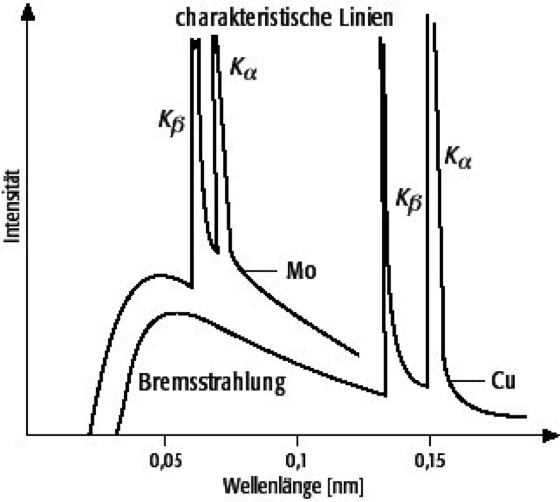
\includegraphics{images/Spektrum_Röntgenröhre.jpg}
                \caption{Spektrum Röntgenröhre [8]}
            \end{figure}

        \subsubsection{Aufbau eines Röntgendiffraktometers}   
            Es gibt verschiedene Aufbauten um Röntgendiffraktogramme zu messen. Der in diesem Versuch verwendete
            Aufbau basiert auf der Bragg-Brentano-Geometrie. Für diesen Aufbau werden flache Proben benötigt, welche in der Mitte
            eines Drehkreises befestigt werden. Die Probe wird mit monochromatischer Röntgenstrahlung bestrahlt, während sich ein
            Detektor auf dem Drehkreis bewegt. Der Detektor fährt eine Strecke 2$\Theta$ ab, wobeo $\Theta$ der Relfexionswinkel bezüglich der reflektierenden Gitterebene. 
            Der Detektor registriert die gebeugten Intensitäten und wandelt diese in elektrische Signale um.
            \begin{figure}[H]
                \centering
                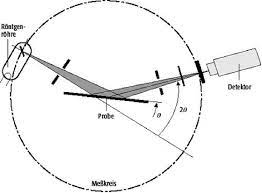
\includegraphics{images/Bragg-Bretano.jpg}
                \caption{Bragg-Bretano-Geometrie [9]}
            \end{figure}

            

        \subsubsection{Intensität der gestreuten Röntgenstrahlung}
            Die Intensität der Röntgenstrahlen ist proportional zum Betragsquadrat des Strukturfaktor. 
            \begin{equation}
                I_{hkl} \propto |F|^2 p L_P A_t
            \end{equation}
            mit F = Strukturfaktor, p = Flächenhäufigkeitsfaktor, $L_P$ = Lorentz-Polarisationsfaktor und $A_T$ = Absorptionsfaktor
            Der Strukturfaktor gibt die Streudichte einer Elementarzelle an. Er lässt sich aus der Fouriertransformierten
            der Ladungsverteilung bestimmen.
            \begin{equation}
                F_{hkl} = \sum_i f_i e^{i \vec{G} \cdot \vec{r_i}}
            \end{equation}
            $\vec{r_i}$ ist der Ortsvektor der i-ten Atoms, $f_i$ der Atomformfaktor und G der reziproke Gittervektor des vorliegenden Bravais-Gitters
            Für ein kubisches Gitter vereinfacht sich  die Formel zu:
            \begin{equation}
                F_{hkl} = \sum_i f_i e^{i 2 \pi (hx + ky + lz)_i}
            \end{equation}
            Für den Strukturfaktor ergibt sich somit, für Cu$_3$Au im geordneten Fall:
            \begin{flalign*}
                F^{g}_{hkl} = f_{Au} \cdot e^{2\pi i (h\cdot 0 + k\cdot 0 + l\cdot 0)} 
                + f_{Cu} \cdot (e^{2\pi i (\frac{h}{2} + \frac{k}{2} + l\cdot 0)} + e^{(2\pi i (\frac{h}{2} + k\cdot 0 + \frac{l}{2})} + e^{(2\pi i (h\cdot 0 + \frac{k}{2} + \frac{l}{2})}) \\
                \Rightarrow F^{g}_{khl} =
                \begin{Bmatrix}
                    f_{Au} + 3f_{Cu}, \text{wenn h,k,l gerade oder ungerade sind}\\
                    f_{Au} - f_{Cu}, sonst
                \end{Bmatrix}
            \end{flalign*}  
            Im ungeordneten Fall gilt:
            \begin{flalign*}
                F^{ug}_{hkl} = (\frac{f_{AU} + 3\cdot f_{Cu}}{4}) \cdot (
                e^{2 \pi i (h\cdot 0 + k \cdot 0 + l \cdot 0)} + e^{2 \pi i (\frac{h}{2} + \frac{k}{2}+ l \cdot 0)}
                + e^{2 \pi i (\frac{h}{2} + k \cdot 0 + \frac{l}{2})} + e^{2 \pi i (h\cdot 0 + \frac{k}{2} + \frac{l}{2})})\\
                \Rightarrow F^{ug}_{khl} =
                \begin{Bmatrix}
                    f_{Au} + 3f_{Cu}, \text{wenn h,k,l gerade oder ungerade sind}\\
                    0, sonst
                \end{Bmatrix}
            \end{flalign*}

            Als Fundamentalreflex werden jene Reflexe bezeichnet, welche im geordneten sowie ungeordneten
            Fall auftreten und identisch sind. Im geordneten Fall treten die sogenannten Überstrukturreflexe
            auf, welche im ungeordneten Fall verboten wären.\\

            Der Lorentz-Polarisationsfaktor ist ein Korrekturterm, welcher die Winkelabhängigkeit der Intensität berücksichtigt. Außerdem,
            dass die beobachteten Peaks keine scharfen Linien bilden.
            \begin{equation}
                L_P = \frac{1 + cos^2(2 \theta)}{8 \cdot sin^2(\theta) cos(\theta)}
                \label{Lorentz-Polarisationsfaktor}
            \end{equation}
            Eine weitere Korrektur ist der Absorptionsfaktor. Er berücksichtigt die Absorption von Strahlung innerhalb des Materials.
            Dieser ist stark von der Probengeometrie abhängig, da die Intensität der Röntgenstrahlung in einer Probe mit
            $$ I = I_0 exp(-\mu d)$$
            $$ \mu = n \sigma$$
            abfällt, dabei beschreibt $\sigma$ den effektiven Wirkungsquerschnitt der Probe, $n$ die Anzahl der Atome pro Kubikmeter und $d$ die Probendicke selbst.
            Um nun den Faktor $A_T$ vernachlässigen zu können, werden stehts nur Reflexe mit kleinem $\theta$ Unterschied verglichen, da
            über Winkelabhängigkeit von $A_T$ so angenommen werden kann, dass $A_T$ für diesen Fall identisch ist.
            
        \subsection{Reflexindizierung im Röntgendiffraktogramm}
            Um die Reflexe im Röntgendiffraktogramm zuordnen zu können lassen sich zunächst mithilfe der Gitterkonstante $a$ für
            kubische Gitter die Netzebenenabstände schreiben als
            \begin{equation}
                d_{hkl} = \frac{a}{\sqrt{h^2+k^2+l^2}}
            \end{equation}
            Da $h,k,l\in \mathbb{N} $ folgt mit
            \begin{equation}
                n\lambda = 2d_{hkl}sin(\theta_{hkl})
            \end{equation}
            , dass sich bei bekannter Wellenlänge so jedem gemessenen Peak, bei Winkel $\theta$, ein Satz millersche Indizes
            zuordnen lässt.
        
    
    \subsection{Die resistive Methode}
        Die zweite Methode zur Proben charakterisierung, die hier Anwendung findet, ist die resistive Methode.
        Dabei erhält man informationen über die Ordnung s im Kristall über die Messung des Widerstands.
        \subsubsection{Elektrische Leitfähigkeit}
            Möchte man die elektrische Leitung von Elektronen durch ein Metall beschreiben bietet sich unter
            anderem das Modell von Arnold Sommerfeld und Paul Drude, auch gennant Drude-Sommerfeld-Modell, an. In diesem Modell
            wird ein elektrischer Leiter mit frei beweglichen Elektronen als Elektronengas betrachtet.
            Durch ein äußeres elektrisches Feld erfahren die freien Elektronen im Leiter eine Kraft $F_{el} = qE$
            und es kommt zu einem Stromfluss. Das Problem der unbegrenzten Beschleunigung wird durch das Drude-Modell
            durch Stöße zwischen den Elektronen und Gitterionen beschrieben, durch die das Elektron abgebremst werden
            und die Energie als Wärme abgegeben wird. Diese Bewegung lässt sich beschreiben über
            \begin{equation}
                ma + \frac{m}{\tau}v_D = -eE
            \end{equation}  
            mit m der Elektronenmasse, v die Elektronengeschwindigkeit, e der Elementarladung, $\tau$ der Stoßzeit, $v_D$ der Driftgeschwindigkeit und E der elektrischen Feldstärke.
            wobei $ma$ die Bewegung ohne Stöße beschreibt und $\frac{m}{\tau}v_D$ genau diese berücksichtigt.
        \subsubsection{Temperaturabhängigkeit}
            Der spezifische Wiederstand einer Kristallstruktur wie z.B. einer Legierung lässt sich schreiben als
            \begin{equation}
                \rho = \rho_D + \rho_L(T)
            \end{equation}
            wobei $\rho_D$ den sogenannten temperaturunabhängigen Restwiderstand und $\rho_L$ den temperaturabhängigen
            Widerstand beschreibt.\\
            Geht man nun von einem reinen Metall zu einer Legierung ändert sich die Gitterstruktur und 
            damit auch die Defektstellen im ursprünglichen Gitter, wodurch über das Phononenspektrum auch
            die Temperaturabhängigkeit beeinflusst wird. Für kleine Konzentrationen an Fremdatomen ist die
            Zahl der zusätzlichen Defektstellen proportional zur Konzentration. Im falle von $Cu_1-_xAu_x$ ergibt sich
            die folgende quadratische Konzentrationsabhängigkeit für den Restwiderstand
            \begin{equation}
                \rho_D(x) = \rho_D(0)+Ax(1-x)
            \end{equation}  
            mit einer Materialkonstante A.\\
            Für Ordnungsfähige legierungen wie $CuAu$ und $Cu_3Au$ muss zusätzlich noch die Abhängigkeit vom
            Ordnungsgrad $S$ der langreichweitigen Ordnung berücksichtigt werden, da diese ebenfalls ein regelmäßiges
            Gitter bilden.
            \begin{equation}
                \rho_D(x) = \rho_D(0)+Ax(1-x)(1-S^2)
            \end{equation}
            Mit bekanntem Restwiderstand und Materialkonstante lässt sich so der Ordnungsparameter bestimmen.
        
        \subsubsection{Vierpunktmethode}   
            Um nun aus dem Widerstand den Ordnungsparameter S zu extrahieren lässt sich die Vierpunktmethode
            zur Widerstandsmessung nutzen. Bei dieser werden vier elektrische Kontakte bzw. Messspitzen auf die 
            Oberfläche gebracht. Nun wird über die äußeren Kontakte ein bekannter/messbarer Strom auf die Oberfläche
            geführt wodurch sich im Material ein elektrisches Feld ausbildet, welches sich in Form einer 
            Potentialdifferenz aus den mittleren Spitzen bestimmen lässt.
            Wichtig bei dieser Messung ist es möglichst weit von den Rändern der Probe entfernt zu sein, da durch die Randbedingungen der
            Strom dort stehts parallel zum Rand fließt. Im Falle der idealisierten Annahme und vier Messspitzen 
            mit gleichem Abstand erhält man den Flächenwiderstand $R_{sq}$ über [3]
            \begin{equation}
                R_{sq} = \frac{\pi}{ln2}\frac{U}{I}
            \end{equation}
            wobei U die Potentialdifferenz der mittleren Spitzen und I der Strom der äusseren Spitzen ist.
            Aus dem Flächenwiderstand lässt sich nun der gewünschte spezifische Widerstand berechnen
            \begin{equation}
                \rho = d R_{sq}
            \end{equation}
            mit d als Schichtdicke der Probe.
